\documentclass{article}

\usepackage{amsmath}
\usepackage[dvips]{graphicx}

\usepackage{natbib}

\bibliographystyle{apa}

\begin{document}

\section{Background}

In multi-class classification, we are choosing between multiple (more than two)
classes based on the results of several binary classifiers.
In what follows, we assume that each binary classifier partitions all $n_c$
classes in different ways and let:
\begin{equation}
r_i=P_i(2|\vec x)-P_i(1|\vec x)
\label{rdef}
\end{equation}
be the difference in conditional probabilities of the $i$th binary classifier.
These conditional probabilities are mapped to the actual probabilities
using a mapping, $A$, which we will call the ``coding matrix'', as follows:
\begin{equation}
\sum_{j=1}^{n_c}a_{ij} p(j|\vec x)=r_i
\label{basic_equation}
\end{equation}
or $A \vec p=\vec r$, where $\vec p=\lbrace p(i|\vec x) \rbrace$ are the conditional probabilities
of the multi-class problem.
The elements of $A$ will be, $a_{ij} \in \lbrace -1, ~1 \rbrace$,
We forbid $A$ from having any zeroes so that all the partitions
partitions divide the whole set of classes, not just a subset--contrast, e.g.,
one-vs.-all and one-vs.-one.
The more complicated case in which zeroes are
allowed will be considered in section \ref{non_strict}.

This looks like a straight-forward linear inverse problem, but with two
caveats.  First, it is frequently over-determined.  Second, it ought to
be constrained: the conditional probabilities 
should always sum to 1:
\begin{equation}
\sum_{j=1}^{n_c} p(j|\vec x) = 1
\label{first_constraint}
\end{equation}
and should also lie between 0 and 1:
\begin{equation}
0 \le p(j|\vec x) \le 1
\end{equation}

Currently the {\it libagf} library \citep{Mills2011},
in the {\it multi-borders} module \citep{Mills2014} solves the 
combination of (\ref{basic_equation}) and (\ref{first_constraint}) via the
normal equation:
\begin{equation}
A^T A \vec p = A^T \vec r
\label{normal_eq}
\end{equation}
where $\vec p=\lbrace p_i \rbrace$, $p_i=p(i|\vec x)$ and the coding matrix,
$A$, includes the constraint in (\ref{first_constraint}) such that 
$a_{n_p+1, j}=1$ for all $j=[1,~n_c]$ and $r_{n_p+1}=1$ where $n_p$ is the total
number of partitions.

\section{Matrix inversion versus voting}

We can contrast two methods of determining the final class.  Matrix inversion:
\begin{equation}
c=\arg \min A^{-1} \vec r
\end{equation}
or, if the matrix is over-determined, a pseudo-inverse such as
the solution to (\ref{normal_eq}):
\begin{equation}
c=\arg \min (A^T A)^{-1}A^T \vec r
\label{pseudoinverse}
\end{equation}
versus voting:
\begin{equation}
c=\arg \min A \vec r
\label{voting}
\end{equation}
with voting being the most popular because it does not require $\vec r$ to
return probabilities but only classes in the form of $\lbrace -1,~+1\rbrace$.
The second form, however, does not produce accurate estimates of the
probabilities.

Why do both forms return accurate estimates of the final class (with tests
suggesting that the second is more accurate), despite the fact that the
role of the variables in the matrix equations are reversed?
First, note that the expression $A^T A$ is always diagonally dominant.
Second, note that it
is quite easy to construct an orthogonal $A$.
For instance, with four classes:
\begin{equation}
A=\left [
\begin{array}{cccc}
-1 & 1 & -1 & 1 \\
-1 & -1 & 1 & 1 \\
-1 & 1 & 1 & -1 \\
1 & 1 & 1 & 1
\label{ortho3}
\end{array}
\right ]
\end{equation}
Here, we have taken $r_4=1$, that is the last row expresses the constraint
in (\ref{first_constraint}).

\section{Case studies}

\begin{figure}
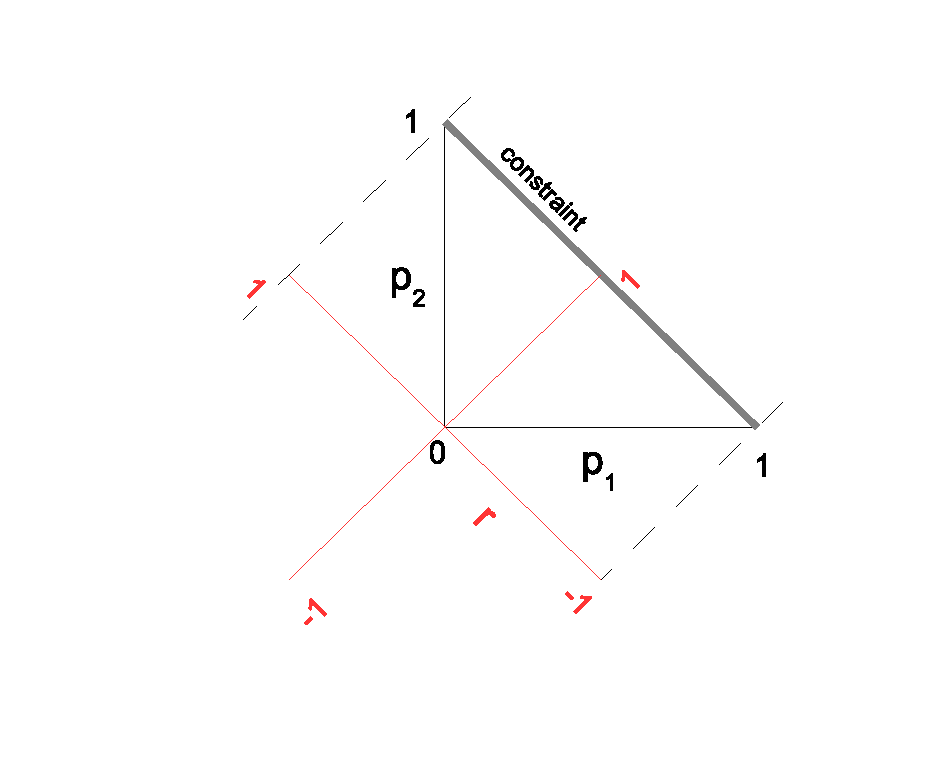
\includegraphics[width=0.9\textwidth]{binary_class_map}
\label{transform}
\end{figure}

Perhaps we can understand the problem better by looking at specific, common 
coding matrices, as the case above suggests.  
The simplest case is a simple, binary classifier with the following 
coding matrix:
\begin{equation}
A = \begin{bmatrix}
-1 & 1 \\
1 & 1
\end{bmatrix}
\end{equation}
including the constraint in (\ref{first_constraint}).  It's useful to think
of the mapping, $A$, as a coordinate transformation as shown in Figure
\ref{transform}.  The final conditional probabilities, $p_1=p(1|\vec x)$ and
$p_2=p(2|\vec x)$, occupy the unit square.  The red lines show the transformed
coordinate system, the first of which is the difference in conditional
probabilities, $r=p_2 - p_1$,
while the heavy grey line is the constraint, $p_1+p_2=1$,
which is constant in the second transformed coordinate.

Next, consider the ``one-vs.-all'' case.  
Using the multi-borders control language
\citep{Mills2014} with $n_c=4$ we can specify it as follows:
\begin{verbatim}
"" 1 2 3 / 0;
"" 0 2 3 / 1;
"" 0 1 3 / 2;
"" 0 1 2 / 3;
\end{verbatim}
The resultant coding matrix will look like this:
\begin{equation}
A = 
\begin{bmatrix}
1 & -1 & -1 & -1 \\
-1 & 1 & -1 & -1 \\
-1 & -1 & 1 & -1 \\
-1 & -1 & -1 & 1 \\
1 & 1 & 1 & 1
\end{bmatrix}
\end{equation}
where, again, we have included the constraint (\ref{first_constraint}) in
the final row.
The squared matrix is given as:
\begin{equation}
A^T A =
\begin{bmatrix}
5 & 1 & 1 & 1 \\
1 & 5 & 1 & 1 \\
1 & 1 & 5 & 1 \\
1 & 1 & 1 & 5 
\end{bmatrix}
\end{equation}

More generally,
\begin{equation}
a_{ij} = \left \lbrace 
\begin{array}{rl}
-1 & | i \ne j \land i \le n_c \\
1 & | i = j \lor i = n_c+1
\end{array}
\right .
\end{equation}
or alternatively:
\begin{equation}
a_{ij} = \left \lbrace 
\begin{array}{rl}
2 \delta_{ij} - 1 & | i \le n_c \\
1 & | i = n_c+1
\end{array}
\right .
\end{equation}
where $\delta$ is the Dirac delta function.
The squared matrix is given:
\begin{equation}
(A^T A)_{ij} = \left \lbrace
\begin{array}{rl}
n_c-3 & | i \ne j \land i \le n_c \\
n_c+1 & | i = j \lor i = n_c+1
\end{array}
\right .
\end{equation}
or:
\begin{equation}
A^T A = 4 I + n_c - 3
\end{equation}
where $I$ is the identity matrix.
But for a multiplicative coefficient and a constant term, this form of coding
matrix is orthogonal.
Thus, we would expect in a one-vs.-all scenario
that the least-squares pseudo-inverse given in 
(\ref{pseudoinverse}) should produce the same solution for the class label
as the voting solution.

Next, we look at the case of class labels running from $1..n_c$ that are 
partitioned between each adjacent class.  For $n_c=4$, the multi-borders
control specification looks like this:
\begin{verbatim}
"" 0 / 1 2 3;
"" 0 1 / 2 3;
"" 0 1 2 / 3;
\end{verbatim}
while the coding matrix looks like this:
\begin{equation}
A = 
\begin{bmatrix}
-1 & 1 & 1 & 1 \\
-1 & -1 & 1 & 1 \\
-1 & -1 & -1 & 1 \\
1 & 1 & 1 & 1
\end{bmatrix}
\end{equation}
and the square is as follows:
\begin{equation}
A^T A =
\begin{bmatrix}
4 & 2 & 0 & -2 \\
2 & 4 & 2 & 0 \\
0 & 2 & 4 & 2 \\
-2 & 0 & 2 & 4 
\end{bmatrix}
\end{equation}
or in the general case:
\begin{equation}
a_{ij} = \left \lbrace 
\begin{array}{rl}
-1 & | i \le j \land i < n_c \\
1 & | i > j \lor i = n_c
\end{array}
\right .
\end{equation}
\begin{equation}
(A^T A)_{ij} = 
n_c-2|i-j|
\end{equation}
This type of partitioning is appropriate for discretized continuous ordinates.

Finally, consider the general case of an orthogonal coding matrix in 
as in (\ref{ortho3}),
which has the property $A^T A = A A^T = n_c I$,
the distance between pairs of both rows and columns will be maximized.
This, according to \citep{Dietterich_Bakiri1995} and
\citep{Allwein_etal2000}, will minimize classification errors. 
An orthogonal matrix, is not trivial to
derive and will not exist for all values of $n_c$.

We can also consider the case of a non-square matrix with $n_p > n_c$,
that nonetheless has the property, $A^T A = n_p I$, where the
identity, $I$, is $n_c \times n_c$. Consider for instance, 
the following matrix for $n_c=5$, 
similar, though not identical, to the ``exhaustive''
matrix described in \citep{Dietterich_Bakiri1995}:
\begin{equation}
  A = 
  \begin{bmatrix}
    1 & -1 & -1 & -1 & -1 \\
    1 &  1 & -1 & -1 & -1 \\
    1 & -1 &  1 & -1 &  1 \\
    1 &  1 &  1 & -1 &  1 \\
    1 & -1 & -1 &  1 &  1 \\
    1 &  1 & -1 &  1 &  1 \\
    1 & -1 &  1 &  1 & -1 \\
    1 &  1 &  1 &  1 & -1 \\
  \end{bmatrix}
\end{equation}
The columns are periodic and thus similar to a set of harmonic functions.
In such case the least-squares ``pseudo''-inverse will equal the voting result
since $(A^T A)^{-1} A^T \cdot \vec r = n_p A^T \vec r$ and the voting method
can return accurate estimates of the conditional probabilities.

\section{``Non-strict'' case}

\label{non_strict}

So far we have only considered the case where the binary classifiers partition
all the classes, but what if we allow the binary classifiers to work with only
a sub-set of all the classes? Now, we allow the coding matrix, $A$, to 
contain $0$ elements: $a_{ij} \in \lbrace -1, 0 1 \rbrace$. 
A $-1$ indicates that the class is in the left side of
the partition, a $1$ that it is in the right side, while a zero means that
it is not included in the partition. 

While the voting method in (\ref{voting}) remains the 
same, the inverse problem in (\ref{basic_equation}) will have to be revised. 
Mainly, we divide
by the sum of the multi-class probabilities contained in the partition:
\begin{equation}
	\frac{\sum_j a_{ij} p_j}{\sum_j |a_{ij}| p_j} = r_i
\end{equation}
where $\vec p$, we recall, is a vector of multi-class conditional probabilities. 
Some rearrangement produces the following:
\begin{equation}
	\sum_j a_{ij} p_j + r_i \sum_{j|a_{ij}=0} p_j = r_i
	\label{general_form}
\end{equation}
Note that this more general formulation includes the ``strict'' case.
To solve the matrix equation in (\ref{general_form}) for the non-strict case, 
the matrix will have to be generated afresh for each estimate
whereas in the strict case, the matrix can be inverted or partially inverted
and then applied to the RHS which is the only part of the equation that
changes.

\section{Re-calibration}

As shown in equation (\ref{rdef}), we summarize the result of a binary
classification using a single variable, $r \in [-1, ~1]$.  For a maximum
likelihood classification, we choose the threshold value for $r$, $r_0$,
that discriminates between the two classes:
\begin{equation}
c = \left \lbrace
\begin{array}{lr}
1 & r<r_0 \\
2 & r>r_0
\end{array}
\right .
\end{equation}
as $r_0 = 0$, but there is no reason why this should be so.  
In both \citep{Mills2009} and \citep{Mills2011}, we show how shifting this
border can be used to recalibrate an image derived from statistical
classification.

Note that because of the constraint in (\ref{first_constraint})
this threshold is equivalent to both a constant value for the conditional
probabilities:
\begin{eqnarray}
r_0 & = & p_2 - p_1 \\
& = & 1 - 2 p_1
\end{eqnarray}
as well as a ratio:
\begin{eqnarray}
f & = & \frac{p_2}{p_1} \\
  & = & \frac{1 - p_1}{p_1}
\end{eqnarray}
Solving for $p_1$ and equating the two produces the following:\
\begin{eqnarray}
p_1 & = & \frac{1}{f+1} = \frac{1 - r_0}{2} \\
r_0 & = & \frac{f-1}{f+1} \\
f & = & \frac{1+r_0}{1-r_0}
\end{eqnarray}

Shifting the threshold can also be used to correct for the case in which we
are training the model using a set of samples whose class statistics
differ from those of the population.
Let $P(1)$ and $P(2)$ be the relative class numbers of the population while
$P^\prime(1)$ and $P^\prime(2)$ are the class numbers of the sample.
Typically, we want:
\begin{equation}
r=P(2|\vec x)-P(1|\vec x)=
\frac{P(2)P(\vec x|2)}{P(\vec x)}-\frac{P(1)P(\vec x|1)}{P(\vec x)} = 0
\end{equation}
or:
\begin{equation}
\frac{P(\vec x|1)}{P(\vec x|2}=\frac{P(2)}{P(1)}
\end{equation}
We want to find an $f$ such that the sample statistics are corrected to
the populations statistics:
\begin{equation}
f = \frac{P^\prime(2)P(\vec x|2)}{P^\prime(1)P(\vec x|1)}
=\frac{P^\prime(2) P(1)}{P^\prime(1) P(2)}
\end{equation}
or:
\begin{equation}
r_0=\frac{P^\prime(2)P(1) - P^\prime(1) P(2)}
	{P^\prime(2)P(1) + P^\prime(1)P(2)}
\end{equation}

\begin{figure}
\includegraphics[width=0.9\textwidth,angle=-90]{rhist.eps}
\caption{Cumulative distribution function (axes reversed) 
of the difference in conditional
probabilities, $r=P(2|\vec x)-P(1|\vec x)$
for the pair of sample classes described in \citet{Mills2011}.}
\label{rhist}
\end{figure}

\begin{figure}
\includegraphics[width=0.9\textwidth,angle=-90]{skillvsr0.eps}
\caption{Two skill scores, accuracy and uncertainty coefficient, as a function of
the decision threshold, $r_0$,
for the pair of sample classes described in \citet{Mills2011}.}
\label{skillvsr0}
\end{figure}

\begin{figure}
\includegraphics[width=0.9\textwidth,angle=-90]{sample_roc.eps}
Receiver operating characteristic (ROC) curve
for the pair of sample classes described in \citet{Mills2011}.
\label{sample_roc}
\end{figure}

In binary classification, the discrimination border can be shifted so as to
optimize any desired skill score.  Since only one parameter is being varied,
the optimization is a straightforward numerical procedure.  Any numerical
minimization technique, such as golden section search \citep{Press_etal1992},
that doesn't require derivatives (which will be discontinuous), can be used.

Figure \ref{rhist} shows the cumulative distribution,
$r$, $F(r)$ for the sample classes discussed in \citet{Mills2011}.  
From this, we can in theory
calculate any skill score for a binary classifier we desire, since:
\begin{eqnarray}
\frac{n_{TP}}{n} & = & \frac{1}{2}\int_{r_0}^{1} (r+1) 
		\frac{\mathrm d F}{\mathrm d r} \mathrm d r \\
\frac{n_{FP}}{n} & = & \frac{1}{2}\int_{r_0}^{1} (1-r) 
		\frac{\mathrm d F}{\mathrm d r} \mathrm d r \\
	& = & F(1) - F(r_0) - \frac{n_{TP}}{n} \\
\frac{n_{TN}}{n} & = & \frac{1}{2}\int_{-1}^{r_0} (1-r) 
		\frac{\mathrm d F}{\mathrm d r} \mathrm d r \\
\frac{n_{TP}}{n} & = & \frac{1}{2}\int_{-1}^{r_0} (r+1) 
		\frac{\mathrm d F}{\mathrm d r} \mathrm d r \\
	& = & F(r_0) - F(-1) - \frac{n_{TN}}{n} 
\end{eqnarray}
where $n_{TP}$, $n_{FP}$, $n_{TN}$, and $n_{FN}$ are the number of true positives
, false positive, true negative and false negatives, respectively, and $n$
is the total number of classes.
[integration by parts...]

The conditional probabilities are calculated based on the definitions of the
probability functions as described in \citet{Mills2011}.  For simple
accuracy, that is, fraction of correct predictions, the optimal decision
threshold should always lie close to zero, assuming the probabilities are
estimated accurately.  For the uncertainty coefficient, which measures the
number of bits of information contained in each prediction
\citep{Shannon, Press_etal1992, Mills2011}, changing the location of the
decision threshold can considerably improve skill scores.  In particular,
if one class is larger than the other, moving the decision border 
{\it closer} to it will typically improve the uncertainty coefficient.
These results are summarized in figure \ref{skillvsr0}.

Finally, the parameter, $r_0$, can also be used to construct 
the receiver operating characteristic (ROC) curve \citep{Jolliffe_Stephenson2003}.
The ROC curve for the pair of sample classes is shown in figure
\ref{sample_roc}.

Presumably, if the classes have been re-calibrated, then the associated 
conditional probabilities need to be transformed also.
Consider the following two transformations:
\begin{equation}
r^\prime = \left \lbrace
\begin{array}{lr}
\frac{r-r_0}{1-r_0} & r<r_0 \\
\frac{r_0-r}{r_0+1} & r>r_0
\end{array} \right \rbrace
\end{equation}
and:
\begin{equation}
r^\prime=\tanh \left (\tanh^{-1}(r)-\tanh^{-1}(r_0) \right ]
\end{equation}
with the second version being similar to what happens after setting the 
\verb/-r/ switch using \verb/class_borders/ in the {\it libagf} package.
Both these have the nice property both that transformed probabilities sum
to one and, if the original probability is one, then so are the transformed
probabilities:
\begin{equation}
p_i^\prime=1 \iff p_i=1
\label{ptop}
\end{equation}

Now consider a simple, linear transformation:
\begin{equation}
\vec p^\prime = A \vec p
\end{equation}
We wish to constrain the transformed probabilities, $\vec p^\prime$,
so that they sum to one as in (\ref{first_constraint}):
\begin{eqnarray}
\sum_i \sum_j a_{ij} p_j & = & 1 \\
\sum_i \sum_j a_{ij} p_j - \sum_j p_j & = & 0 \\
\sum_j p_j \left (\sum_i a_{ij} - 1 \right ) & = & 0
\end{eqnarray}
Thus all the columns of the transformation matrix must also sum to one:
\begin{equation}
\sum_i a_{ij} = 1
\end{equation}
In other words, the transformation matrix, $A$, is itself a conditional
probability.  If we wish to keep the constraint in (\ref{ptop}) then the only
solution is the identity matrix, $I$.


\section{Constrained problem}

\begin{figure}
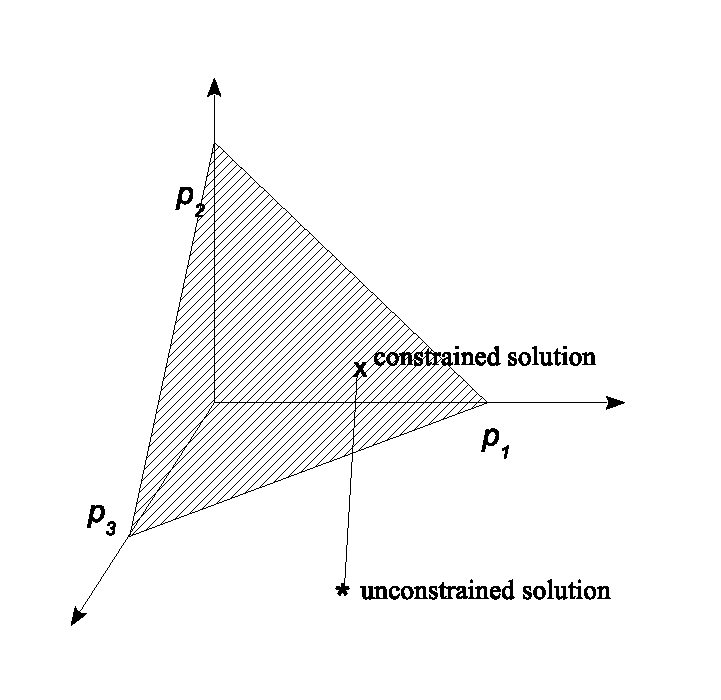
\includegraphics[width=0.9\textwidth]{config1}
\label{fig1}
\end{figure}

We wish to solve the following minimization problem:
\begin{equation}
\underset{\vec p}{\min} (A \vec p - \vec r)^2 
\end{equation}
subject to the constraints:
\begin{eqnarray}
\sum_{i=1}{n_c} & p_i & = 1 \\
0 \le & p_i & \le 1; ~i=0..n_c
\end{eqnarray}
The situation is illustrated in Figure \ref{fig1} for the case of three classes.

The first constraint is easily applied by a change of variables, e.g.:
\begin{equation}
p_j=1-\sum_{i \ne j} p_i
\end{equation}
reducing the dimensionality of the problem by one. 

Also with a change of variables: 
\begin{equation}
\vec x = A \vec p - \vec r
\end{equation}
we can transform the minimization problem into
something quite trivial:
\begin{equation}
\underset{\vec x}{\min} {\vec x}^2
\label{trivial_min}
\end{equation}
After applying the first constraint, the problem in the transformed coordinates
becomes a matter of finding the point closest to the origin on or in the 
triangular hyper-pyramid defined by the rest of the constraints.

Once we've made these two transformations, it makes sense to make the constraints
more general.  There are a number of ways of specifying a triangular
hyper-pyramid.  The most obvious is with a series ($n_c$ in this case) of hyper-
planes:
\begin{equation}
	\vec v_i \cdot \vec x - b_i > 0 ~ | ~ i=[1, ~n_c]
\label{generalized_constraint}
\end{equation}
Here we have switched to $\vec x \in \Re^{n_c-1}$ as the solution variable.  These can be 
converted to a series of $n_c$ vertices.  By ommitting one of the constraints
and converting the remaining to a system of linear equations:
\begin{equation}
\vec v_i \cdot \vec c_j = b_i | ~ i \ne j
\end{equation}
we can solve for the vertex, $\vec c_j$, opposite the hyperplane defined 
by the $j$th constraint.

Likewise, we can return to the format in (\ref{generalized_constraint}) via the
generalized cross-product or wedge product:
\begin{eqnarray}
	\vec v_i^\prime & = & \wedge \left ( \lbrace \vec c_j - \vec c_{j-1} | j \ne i \rbrace,~ \vec c_1-\vec c_{n_c} \right ) \\
	b_i^\prime &= & \vec v_i^\prime \cdot \vec c_j | ~ i \ne j \\
	d & = & \mathrm{sgn} \left (\vec v_i^\prime \cdot \vec c_i - b_i^\prime) \right ) \\
	\vec v_i & = & d \vec v_i^\prime \\
	b_i & = & d b_i^\prime \\
\end{eqnarray}
[is this correct?]

To solve the basic minimization problem in (\ref{trivial_min}) subject to
one of the constraints, simply connect the hyperplane with the origin via
the normal, $\vec v_i$:
\begin{eqnarray}
	\vec x_{min} & = & t \vec v_i \\
	t \vec v_i \cdot \vec v_i & = & b_i \\
	t & = & \frac{b_i}{|\vec v_i|^2} \\
	\vec x_{min} & = & \frac{b_i}{|\vec v_i |^2} \vec v_i \label{solution_1constraint}
\end{eqnarray}

To show that this satisfies (\ref{trivial_min}) we can rearrange the constraint
to solve for one of the variables:
\begin{equation}
	\vec x_i = b - \sum_{j \ne i} v_j x_j
\end{equation}
where for simplicity we have omitted the subscript enumerating the constraint
from the parameters.
Substituting this into the minimization problem:
\begin{equation}
	\vec x \cdot \vec x = \sum_{j \ne i} x_j^2 + 
	\left (\frac{b}{v_i} - \frac{1}{v_i} \sum_{j \ne i} v_j x_j \right )^2
\end{equation}
Minimizing this expression:
\begin{eqnarray}
	\frac{\partial}{\partial x_k} \vec x \cdot \vec x = 2 x_k - 2 \frac{v_k}{v_i} \left (\frac{b}{v_i} - \frac{1}{v_i} \sum_{j \ne i} v_j x_j \right )^2 
	& = & 0 \\
	\frac{v_i}{v_k} x_k - \frac{b}{v_i^2} + \sum{j \ne i} v_j x_j & = & 0
	\label{min_1constraint}
\end{eqnarray}
Substituting (\ref{solution_1constraint}) into (\ref{min_1constraint})
produces the following:
\begin{equation}
	\frac{v_i^2 b}{|\vec v|^2} - b + \frac{b}{|\vec v|^2} \sum_{j \ne i} v_j^2 
    = \frac{b}{|\vec v|^2} \left (\sum_{j \ne i} v_j^2 + v_i^2 \right ) - b = 0
\end{equation}

\section{Solving the constrained problem}

We wish to solve the following minimization problem:
\begin{equation}
	\arg \min_{\vec x} |\vec x|
\end{equation}
where $\vec x \in \Re^n$, subject to the following constraints:
\begin{equation}
	\vec v_i \cdot \vec x \ge c_i
\end{equation}
where $i \in [1, n+1]$ and the constraints enclose a hyper-pyramid.

Since both the minimization problem and the constraints are convex 
\citep{Boyd_etal2004}, the basic procedure is first, to find the unconstrained
solution, then find an interior point and move towards the unconstrained
solution. If we encounter a constraint, then we restrict the solution so as
to lie along the constraint and continue to move towards the unconstrained
solution. We outline the steps in detail below.

\subsection{Step 1: finding the interior point}

Let $V_k$ be the matrix containing the set of constraint normals but
excluding the $k$th normal: $V_k = \lbrace \vec v_i | i \ne j \rbrace$. 
We first transform the problem by letting $\vec z=V_k \cdot \vec x$.
Let $\vec z_0 = \lbrace c_i | i \ne k \rbrace$.

We are searching for an interior point, 
$\vec p = V_k^{-1} \cdot \vec z_0 + \Delta \vec x$, 
where $\Delta \vec x$ has only positive components, such that:
\begin{equation}
	\vec v_k \cdot \left ( V_k^{-1} \cdot \vec z_0 + \Delta \vec x \right ) > c_k
\end{equation}
If the constraints have been laid out properly, the inequality should be 
satisfied when $\Delta \vec x$ is zero.
We can't solve for $\Delta \vec x$ directly since it can take on a 
multitude of different values. What we can do is
take the difference between the left and right sides with $\Delta \vec x = \vec 0$
\begin{equation}
	d = \vec v_k \cdot V_k^{-1} \cdot \vec z_0 - c_k
\end{equation}
and spread some fraction, $f;~0 < f < 1$, of this difference evenly between the 
elements of the interior point, $\vec p$:
\begin{equation}
	\vec p = V_k^{-1} \cdot \vec z_0 + \frac{f d}{\vec v_k \cdot \vec 1} \vec 1
\end{equation}
where $\vec 1$ is a vector of ones.

\subsection{Step 2: move between the interior point and the unconstrained solution}

Let $\vec x_0$ be the unconstrained solution. Initially, this will simply be
the zero vector, $\vec x_0 = \vec 0$, but will change with successive 
refinements to the solution. See below. 

Either this solution violates no constraints,
in which case no further work needs to be done, or
it violates one or more of them. In the latter case, we find, for each of the
violated constraints, the distance
to the constraint hyper-plane along the line between the interior point and
the unconstrained solution:
\begin{equation}
	s_i = \frac{c_i - \vec v_i \cdot \vec p}
	{\vec v_i \cdot \vec x_0 - \vec v_i \cdot \vec p}
\end{equation}
where $s_i$ is the line parameter and
$\lbrace i |~\vec v_i \cdot \vec x_0 < c_i \rbrace$ are the violated
constraints. Again if the constraints have been laid out properly, $s$ should
always be positive.


Let $s_{min}=\min_i s_i$ be the minimum value for the line parameter and 
$h=\arg \min_i s_i$ be the closest violated constraint.
If $n=1$ then the solution is $x=\frac{c_h}{v_h}$

\subsection{Step 3: restrict the problem to lie on the closest violated constraint}

Let $k$ be an index for $\vec x$ such that $v_{jk} \ne 0$. 
We eliminate $x_k$ using the following transformation:
\begin{equation}
	x_k = \frac{c_h - \sum_{i \ne k} v_{hi} x_i}{v_{hk}}
\end{equation}
Therefore, each of the constraints transform as follows:
\begin{eqnarray}
	v_{ij}^\prime & = & \left \lbrace \begin{array}{rc} 
	v_{ij} - \frac{v_{hj}}{v_{hk}} ; & j < k \\
	v_{ij+1} - \frac{v_{hj+1}}{v_{hk}} ; & j \ge k
	\end{array} \right . \\
	c_i^\prime & = & c_i - \frac{c_h}{v_{hk}} \\
	i & \ne & h \\
	j & \in & [1, n-1]
\end{eqnarray}
Note that the problem is now reduced in size by one.

\subsection{Step 4: find the new interior point and unconstrained solution}

The new interior point can be found using the line parameter, $s_{min}$:
\begin{equation}
	\vec p^\prime = \vec p + s_{min} (\vec x_0 - \vec p)
\end{equation}
The new value for $x_0$ is the closest point to the old value inside the
constraint hyper-plane:
\begin{equation}
	\vec x_0^\prime = \vec x_0 + \left ( \frac{c_h - \vec v_h \cdot \vec x_0}{| \vec v_h |^2} \right ) \vec v_h
\end{equation}
Using these vectors with the $k$th component eliminated, we restart the
solution from Step 2.


\bibliography{../agf_bib.bib} 

\end{document}
